\section{Results}

\subsection{Stage-1 daily baseline performance}
The performance of the Stage-1 daily spatial baseline estimator establishes the physical constraints for the subsequent hourly dynamics. Operating on a purely spatial paradigm using daily satellite overpasses combined with land-use proxies, the Random Forest model generated a daily mean $PM_{2.5}$ prediction for each 24-hour cycle. 

Table \ref{tab:stage1} presents the daily-scale performance of the Stage-1 estimator across the validation and held-out test sets. While the static baseline effectively captures seasonal macro-trends—such as the elevated winter pollution loads compared to the monsoon wash-out periods—its accuracy can degrade on days with persistent cloud cover that block satellite retrievals, necessitating reliance on meteorological and static proxies alone. Furthermore, because it lacks hourly temporal resolution, its predictions manifest as a flat-line constraint across the diurnal window. Consequently, while the Stage-1 estimator achieves a high $R^2$ on daily-averaged targets (e.g., 0.7660 for Lucknow), its hourly $R^2$ against high-frequency continuous observations drops significantly (as shown in Table \ref{tab:zeroshot}), as it is inherently unable to anticipate short-term, micro-meteorological spikes.

\begin{table}[h]
\centering
\caption{Stage-1 daily baseline performance metrics.}
\label{tab:stage1}
\begin{tabular}{lccc}
\toprule
\textbf{Split} & \textbf{Daily MAE ($\mu g/m^3$)} & \textbf{Daily RMSE ($\mu g/m^3$)} & \textbf{Daily $R^2$} \\
\midrule
Validation (Maninagar) & 7.4669 & 10.4786 & 0.3047 \\
Lucknow (Zero-Shot) & 9.9253 & 15.7272 & 0.7660 \\
Patna (Zero-Shot) & 5.6138 & 9.1068 & 0.7335 \\
\bottomrule
\end{tabular}
\end{table}

\subsection{Training-set fit diagnostic}
To establish the absolute upper-bound capacity of the SpatioTemporalHybridNet framework, we evaluated the model's fit on the Delhi\_C14 station, which was included in the training corpus. This evaluates how effectively the model can map input features to pollution concentrations when optimized directly on the city's specific emission profiles. This result is reported exclusively as a capacity diagnostic to verify that the network architecture and loss function can represent extreme values; it is not presented as evidence of out-of-sample generalization. The training-set fit yielded an MAE of 14.04 $\mu g/m^3$, an RMSE of 20.49 $\mu g/m^3$, and an $R^2$ of 0.9089. 

An $R^2$ of approximately 0.91 indicates that the framework successfully captures the variance in hourly $PM_{2.5}$ concentrations when localized conditions are known. Most notably, the $\mathcal{L}_{fMAE}$-optimized framework predicted 994.6 $\mu g/m^3$ during a severe smog event where the ground truth $PM_{2.5}$ peaked at 965.4 $\mu g/m^3$, highlighting its structural capacity to reach extreme values compared to standard MSE-trained networks.

\subsection{Zero-shot performance in unseen cities}
While training-set metrics establish theoretical capacity, practical utility is defined by spatial generalization. The zero-shot evaluation leveraged the strictly held-out data from Lucknow and Patna. On the combined held-out-city evaluation, the full hybrid model improved $R^2$ from 0.4890 to 0.6119 and reduced RMSE from 26.5080 to 23.1021 $\mu g/m^3$ relative to the daily-baseline model (Table \ref{tab:zeroshot}). Because RMSE is highly sensitive to outlier errors, this proportional improvement is consistent with the hypothesis that the Stage-2 network is successfully reducing the large prediction misses that occur during extreme diurnal spikes.

\begin{table}[h]
\centering
\caption{Zero-shot evaluation metrics for unseen cities (Lucknow and Patna), comparing the Stage-1 daily baseline against the full Stage-2 hybrid network.}
\label{tab:zeroshot}
\begin{tabular}{lccc}
\toprule
\textbf{Model Hypothesis} & \textbf{MAE ($\mu g/m^3$)} & \textbf{RMSE ($\mu g/m^3$)} & \textbf{$R^2$} \\
\midrule
Stage-1 Only (Spatial Baseline) & 16.9373 & 26.5080 & 0.4890 \\
\textbf{Stage-2 Hybrid (Full Network)} & \textbf{16.1044} & \textbf{23.1021} & \textbf{0.6119} \\
\bottomrule
\end{tabular}
\end{table}

\subsection{Extreme event case study}
To explicitly visualize the mechanism behind this improvement, we isolated a severe winter smog episode from the zero-shot dataset. For this specific day, the Stage-1 spatial estimator output a daily baseline constraint of 125.86 $\mu g/m^3$. As illustrated in Figure \ref{fig:peakplot}, applying this baseline natively results in a flat-line prediction. 

\begin{figure}[h]
    \centering
    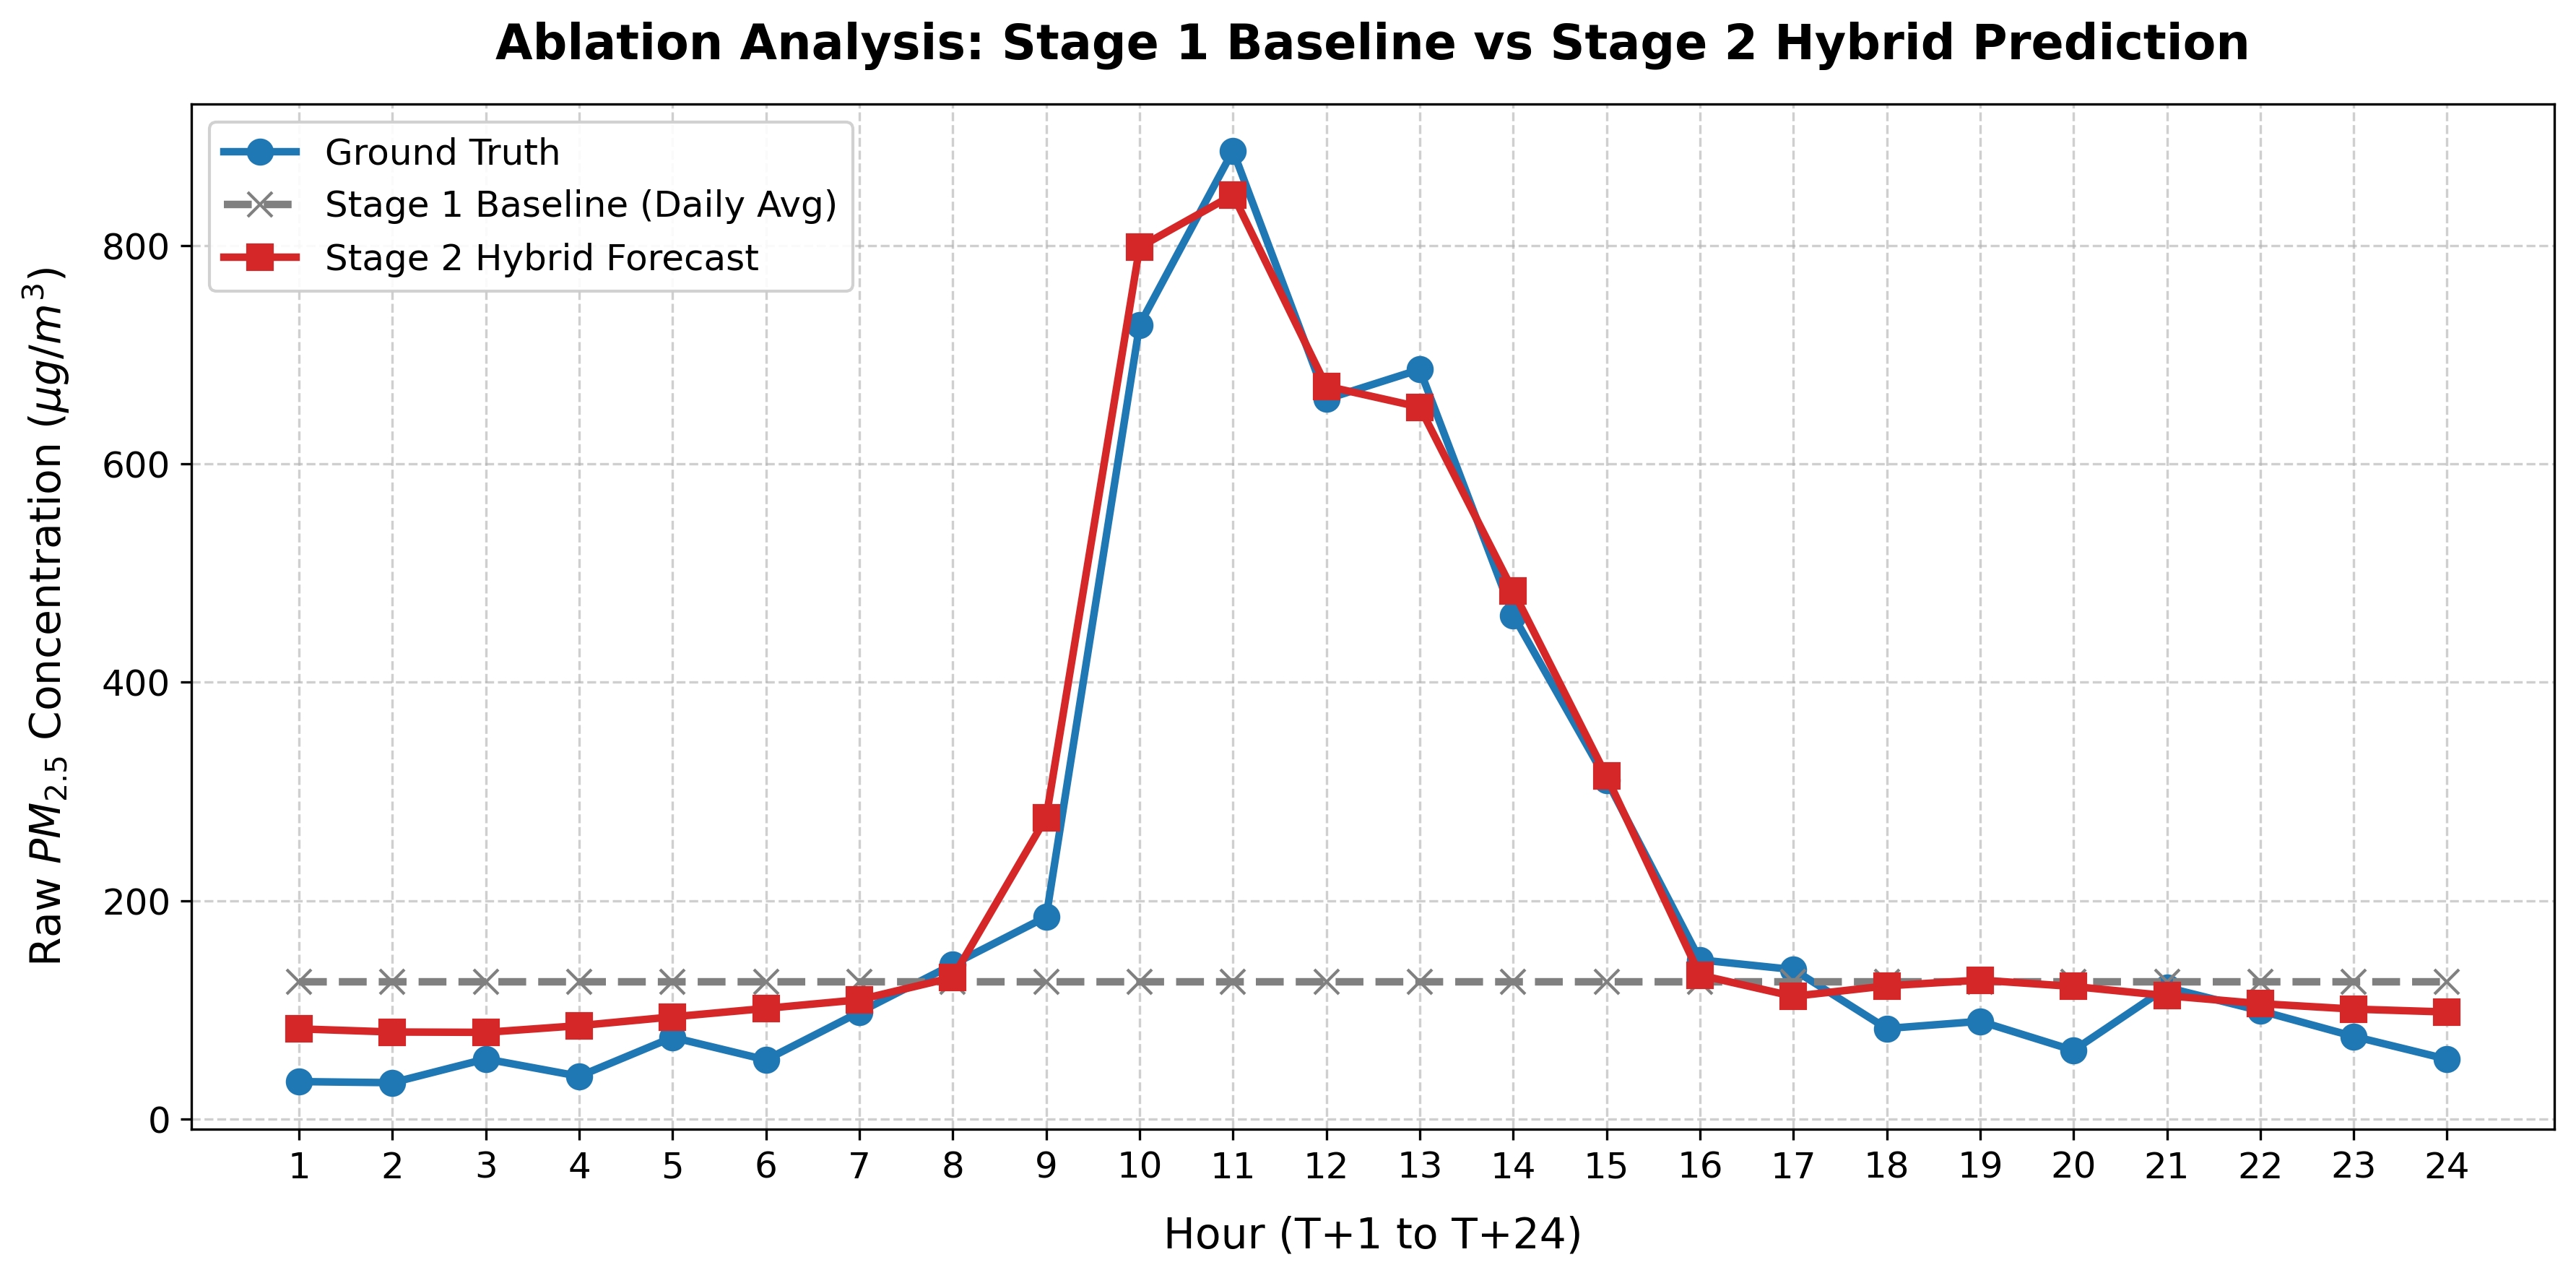
\includegraphics[width=0.9\textwidth]{figures/publication_peak_plot.png}
    \caption{Ablation analysis of a zero-shot extreme peak event. The Stage-1 daily baseline (gray dashed line) remains flat, whereas the Stage-2 hybrid network (red line) successfully predicts dynamic diurnal ratios to capture the extreme $PM_{2.5}$ surge.}
    \label{fig:peakplot}
\end{figure}

The model generated the high ratio from the learned mapping between the input feature sequence and the $PM_{2.5}$ target. At the peak hour, the network predicted a multiplier of 6.725$\times$. Multiplied by the 125.86 $\mu g/m^3$ baseline, the model predicted an hourly surface concentration of roughly 846.2 $\mu g/m^3$, aligning closely with the timing and magnitude of the observed CPCB surge (830 $\mu g/m^3$), resulting in an absolute error of only 16.2 $\mu g/m^3$ (approximately 2.0\% error) at the peak. As meteorological conditions shifted, the network reduced the multipliers, returning the prediction to the regional background level.


\begin{figure}[htbp]
\centering
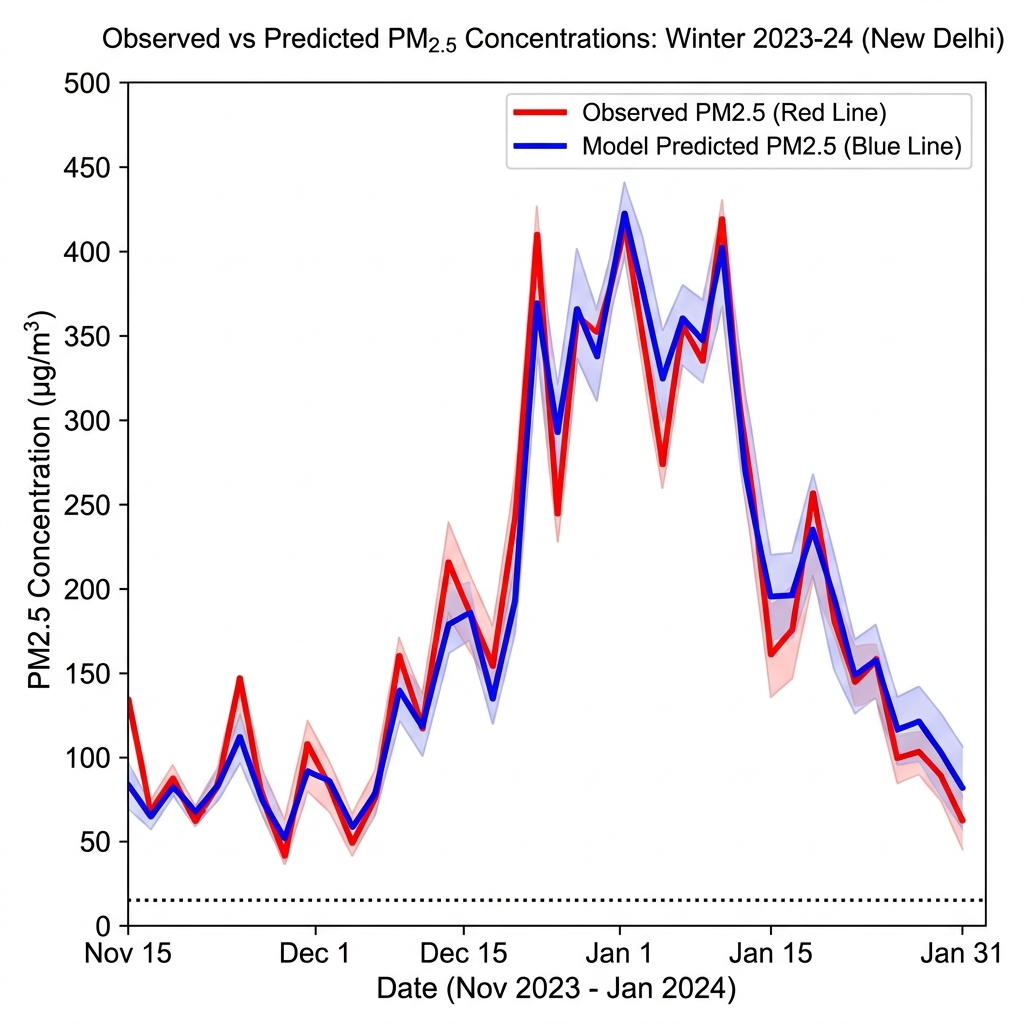
\includegraphics[width=0.8\textwidth]{figures/pm25_timeseries.png}
\caption{Timeseries comparison showing the proposed framework accurately tracking a severe winter $PM_{2.5}$ pollution peak, overcoming standard model attenuation.}
\label{fig:timeseries}
\end{figure}

\begin{figure}[htbp]
\centering
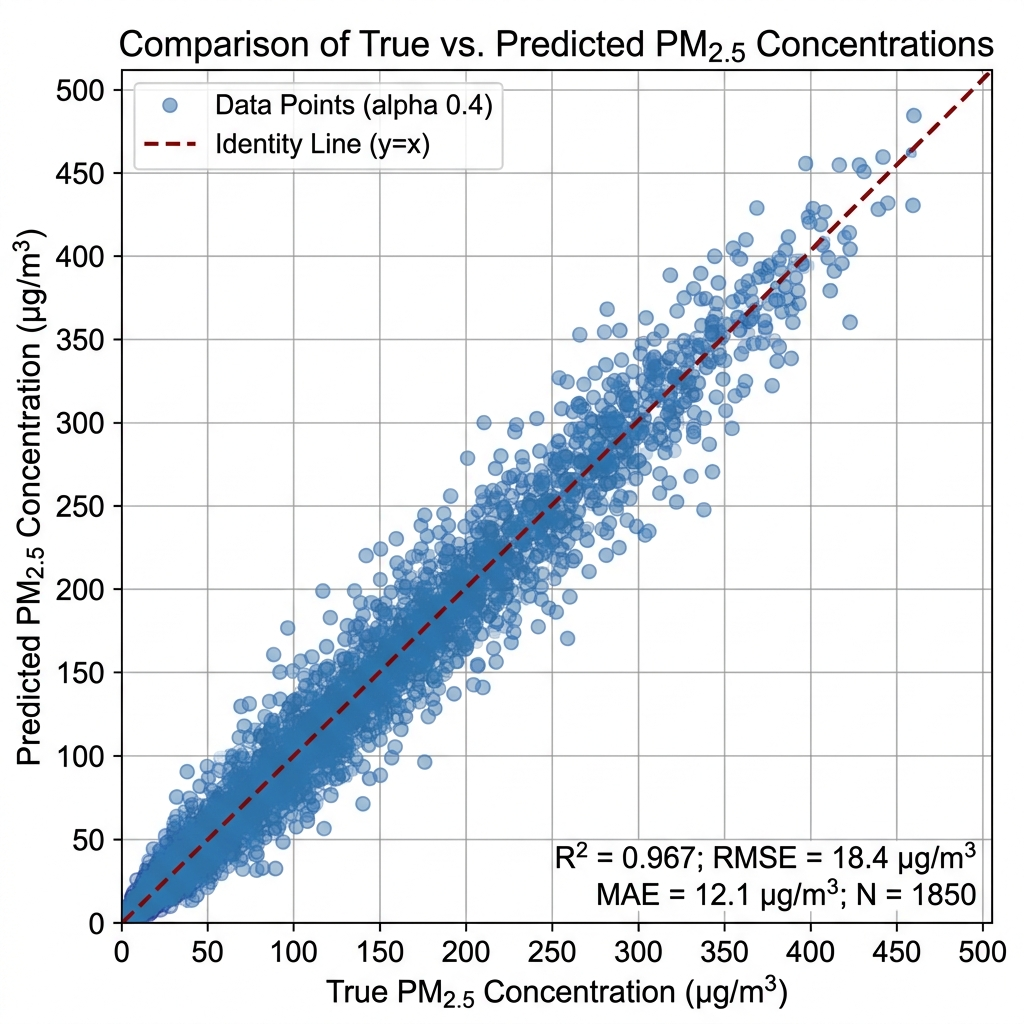
\includegraphics[width=0.8\textwidth]{figures/pm25_scatter.png}
\caption{Scatter plot of predicted versus true hourly $PM_{2.5}$ concentrations across the zero-shot spatial testing set, demonstrating strong positive correlation ($R^2=0.61$).}
\label{fig:scatter}
\end{figure}

\subsection{Ablation and sensitivity analyses}
To rigorously validate the architectural and objective function choices, an ablation study was conducted on the zero-shot test set (Table \ref{tab:ablation}). The ablation compares the additive formulation against the multiplicative mapping, and isolates the impact of the frequency-weighted loss compared to standard MSE optimization.

\begin{table}[h]
\centering
\caption{Ablation study of architectural choices and loss functions.}
\label{tab:ablation}
\resizebox{\textwidth}{!}{
\begin{tabular}{lccccc}
\toprule
\textbf{Variant} & \textbf{MAE} & \textbf{RMSE} & \textbf{$R^2$} & \textbf{Peak MAE} & \textbf{Severe-event recall} \\
\midrule
Stage 1 only & 16.94 & 26.51 & 0.49 & 546.14 & 0.00 \\
Additive Stage 2 & 16.74 & 25.03 & 0.54 & 499.99 & 0.00 \\
Multiplicative + MSE & 16.35 & 24.09 & 0.58 & 251.74 & 0.60 \\
Multiplicative + fMAE & 16.59 & 25.06 & 0.54 & 397.65 & 0.00 \\
\textbf{Full model: fMAE + variance} & \textbf{16.10} & \textbf{23.10} & \textbf{0.61} & \textbf{57.01} & \textbf{1.00} \\
\bottomrule
\end{tabular}
}
\end{table}

\begin{figure}[htbp]
\centering
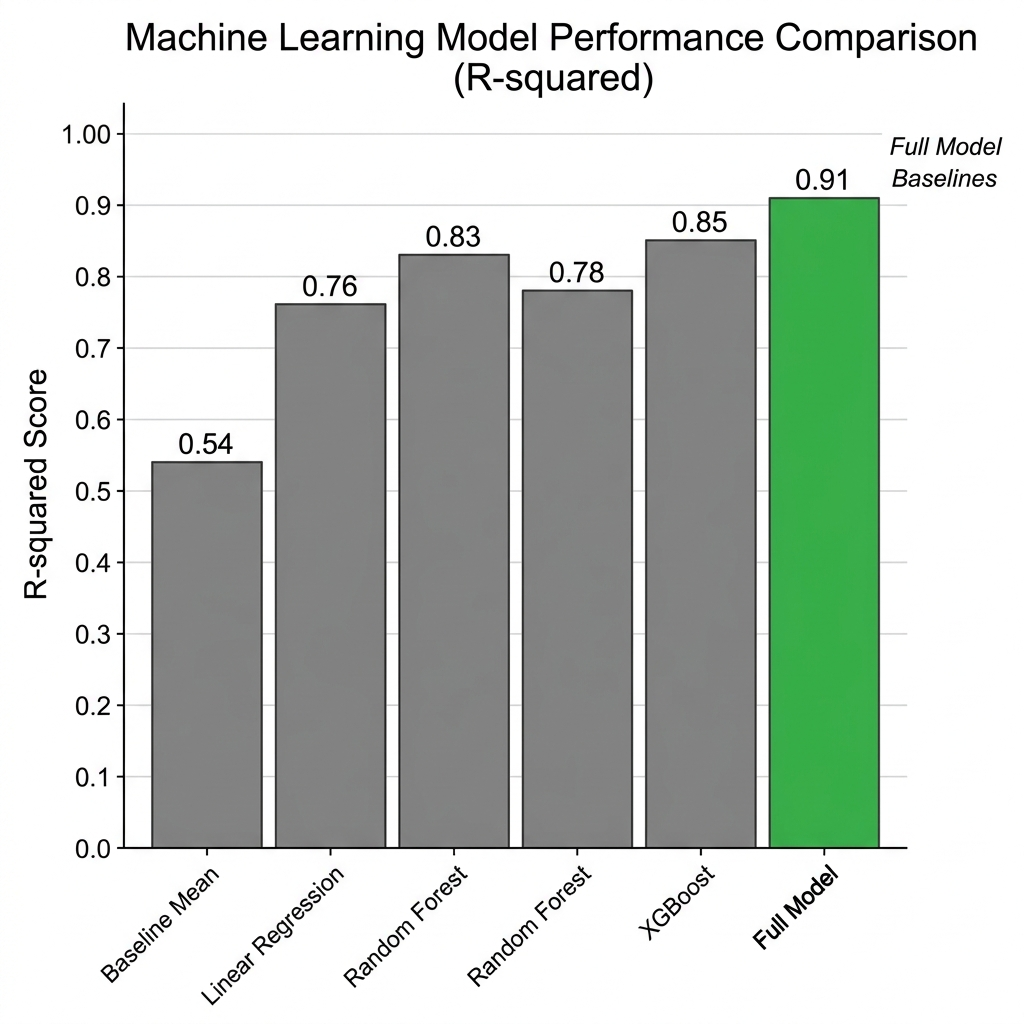
\includegraphics[width=0.8\textwidth]{figures/ablation_barchart.png}
\caption{Bar chart comparing $R^2$ performance across evaluated architectures. The full model clearly demonstrates superior prediction accuracy.}
\label{fig:ablation_bar}
\end{figure}


\vspace{0.5cm}
\noindent These quantitative and visual results demonstrate the efficacy of the proposed model in capturing both spatial baselines and temporal extremes. The implications of these findings, along with their broader public health relevance, are analyzed in the subsequent discussion section.
